\documentclass[10pt]{article}

\usepackage{amsmath}
\usepackage{amssymb}
\usepackage{graphicx}
%\usepackage{picins}
\usepackage{amsthm}
\usepackage{bbm}

\setlength{\voffset}{-28.4mm}
\setlength{\hoffset}{-1in}
\setlength{\topmargin}{20mm}
\setlength{\oddsidemargin}{25mm}
\setlength{\evensidemargin}{25mm}
\setlength{\textwidth}{160mm}
\usepackage{subfigure}
\usepackage{fixltx2e}
\setlength{\parindent}{0pt}

\setlength{\textheight}{210mm}
%\setlength{\footskip}{20mm}
\setlength{\headsep}{50pt}
\setlength{\headheight}{0pt}

% Paket zur Verwendung einer verbesserten Schriftart
\usepackage{lmodern}

%Language package französisch
\usepackage[english]{babel}
\usepackage[T1]{fontenc}
\usepackage[utf8]{inputenc}

\usepackage{wrapfig}

%Hyperref
\usepackage[backref = true]{hyperref}

%Einbinden von Graphen
\usepackage{tikz}

%für die pc schriftart 


\begin{document}
	
\begin{titlepage}
	\begin{center}
	
		{\Large
			Université de Pierre et Marie Curie \\[5mm]
		}
		\normalsize
		\medskip
		
		{\large
			Course Project 'Initiation au C++'\\[20mm]
			}
		
		
		{\Huge
			Fast search of a triangle covering\\ a point in a mesh
		}
		\vspace{2cm}
		
		\normalsize
		
		{\Large
		Arne Heimendahl, Olivia Kaufmann	
			}
		
		
		\begin{figure}[t]
			\begin{center}
			
\includegraphics[width=0.5\linewidth]{UPMC_Sorbonne_Universites.png}	
			\end{center}
		\end{figure}
		
	\end{center}
	\vspace*{60mm}
	
	{\large
		Supervisor: F. Hecht, X. Claeys\\[3mm]

		Submission Date: 11/01/2018 
	}
	
	
	
\end{titlepage}

\newpage
\tableofcontents
\newpage

%\pagenumbering{arabic}
%\pagestyle{headings}
	
%\title{Recherche rapide d’un triangle contenant un point dans un maillage}

\begin{wrapfigure}{r}{0.4\textwidth} \label{fig:ex_mesh}
	\begin{center}
		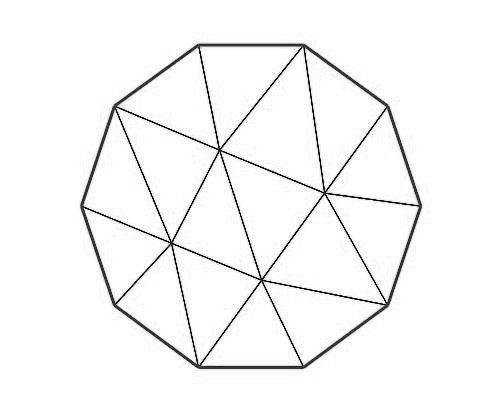
\includegraphics[width=0.6\linewidth]{../Figures/ex_mesh}
	\end{center}
	\caption{Example for a mesh}
\end{wrapfigure}

\section{Project description and aim}

The aim of this project is to implement an algorithm which searches for a triangle in a convexe mesh covering a point $p = (x,y)$. A linear complexity in number of vertices of the mesh is desired.

A mesh is a set of triangles where the intersection of two triangles is either empty, a vertex or an edge. See Figure \ref{fig:ex_mesh} for an illustration.

\begin{enumerate}
	\item The task is to implement a class {\ttfamily Mesh} who stores arrays of vertices and triangles. The data shall be imported from a mesh file.
	\item A function given an input triangle and one of its vertices returning an adjacent triangle opposite to the vertex shall be implemented. The complexity should be constant after an unique initialization  of the neighbors in $O(n_T)$ or $O(n_T \log(n_T))$.
	\item An algorithm starting in a given triangle and walking until finding the covering triangle of a specified point is demanded.
	\item Thereafter, the results shall be displayed.
	\item Given two meshes, {\ttfamily m} and {\ttfamily M}, covering triangles in {\ttfamily M} of the vertex set of {\ttfamily m} shall be searched.
\end{enumerate}

\section{The template class T3 and the class Triangle}

\subsection{The template class T3} \label{T3}

Objects of the class {\ttfamily T3} represent elements of a three dimensional space in {\ttfamily T}. Hereby, the data type {\ttfamily T} is defined using a template. Within this project, either {\ttfamily T3<int>} for the definition of a triangle (see \ref{triangle}) or {\ttfamily T3<double>} for the definition of the coordinates of a vertex (see \ref{mesh}) is used. The private members $x,y$ and $z$ of type {\ttfamily T} store the entries of the {\ttfamily T3} vector. The class has a default constructor, a constructor by copy and a constructor creating a vector given the three vector entries. Moreover, the class has operators to access and modify the entries, add to elements of {\ttfamily T3}, multiply an element of {\ttfamily T3} by a scalar of the type {\ttfamily T} and calculate the scalar product of two {\ttfamily T3} vectors. The operator $<$ compares two elements of {\ttfamily T3}, $v_1 = \begin{pmatrix} x_1 & y_1 & z_1 \end{pmatrix}^T$ and $v_2 = \begin{pmatrix} x_2 & y_2 & z_2 \end{pmatrix}^T$, in the following way:
$$ v_1 < v_2 \quad \Leftrightarrow \quad \begin{cases}
 x_1 < x_2 \text{ or }\\
 x_1 = x_2 \text{ and } y_1 < y_2 \text{ or }\\
 x_1 = x_2 \text{ and } y_1 = y_2 \text{ and } z_1 < z_2
\end{cases}. $$ 
This allows a lexicographic ordering of a list of {\ttfamily T3} elements (see \ref{list}, {\ttfamily T3<int>}). For three {\ttfamily T3} vectors, which define the vertices of a triangle, the method {\ttfamily T3::oriented\_vol } computes the corresponding signed volume. Let $a,b$ and $c$ denote {\ttfamily T3} vectors. The {\itshape oriented volume }is defined as
$$ \left( \overrightarrow{ab} \times \overrightarrow{bc} \right)^T \begin{pmatrix} 0 \\ 0 \\ 1 \end{pmatrix} = (b_1-a_1)(c_2-b_2) - (b_2-a_2)(c_1-b_1)$$

The sign is positive for triangles oriented in trigonometric sense. This method is used in the method {\ttfamily Mesh::Promenade} \ref{promenade} to determine a suitable 'walking' direction.


\subsection{The class Triangle} \label{triangle}
The class {\ttfamily Triangle} inherits form the class {\ttfamily T3}. Its derived members $ i,j,k $ are specialized as integers representing the position of its defining vertices in the array of the points of the given mesh. This array is a member of the class {\ttfamily Mesh} in \ref{mesh}. In addition, it has three extra integer members {\ttfamily Triangle::int neighbor1, neighbor2, neighbor3} representing the position of the adjacent triangles in the array of triangles which is also a member of the class {\ttfamily Mesh}. Notice that theses index lies between zero and the number of triangles minus one. \\
 An adjacent triangle $ t^{'} $ is said to be  {\ttfamily neighbor1} of a triangle $ t $ if, saying $ i $ represents the first index of a vertex of $t$ but $i$ does not represent a vertex of $ t^{'} $. The same holds for {\ttfamily neighbor1} and {\ttfamily neighbor2}. Note that this relation is not symmetric, that is to say that $ t^{'} $ is {\ttfamily neighbor1} does not imply that $t$ is {\ttfamily neighbor1} of $t^{'}$. 
This assignment facilitates the access to the following adjacent triangle in the algorithm {\ttfamily Promenade} (see \ref{promenade}).  \\
At the creation of a new triangle the latter three members are initialized by $ -1 $ which means that a triangle has no neighbors when it is created. The functions {\ttfamily Mesh::setAdjacencyViaMultimap} (see \ref{multimap}) and {\ttfamily Mesh::setAdjacencyViaList} (see \ref{list}) set the neighbors via the stl containers multimap, respectively list. After the execution of one of these two functions {\ttfamily neighbor1 $ = -1$} describes the case that there is no adjacent triangle on the opposite side of the first vertex. 
Since the neighbors are private members there are getter and setter in order to read and manipulate them.

\section{The class Mesh} \label{mesh}
The class {\ttfamily Mesh} contains all necessary information of the mesh and the search of a vertex in (or outside) the mesh can be realized by its member functions. Its private members are pointers to the arrays of vertices and triangles of the mesh as integers who store the size of these two lists.
In order to create an object of type {\ttfamily Mesh} the name of the desired .msh file has to be transmitted. The file is read by the functions {\ttfamily Mesh::LoadVertices} and {\ttfamily Mesh::LoadTriangles} \ref{Load} who then initialize the members {\ttfamily Mesh:: Triangle* triangles, T3<double> vertices, int numbTriangles, int numbVertices}.
Since the members are private there are getter and setter for {\ttfamily numbTriangles} and {\ttfamily numbVertices} as well as getter for {\ttfamily triangles} and {\ttfamily vertices}. The functions {\ttfamily LoadTriangles} and {\ttfamily LoadVertices} are their setters.


\subsection{LoadVertices and LoadTriangles} \label{Load}
Both functions are called in the constructor of the class {\ttfamily Mesh} setting the members {\ttfamily vertices} and {\ttfamily triangles}.
They work basically the same way with the small difference that they create arrays of different data types ({\ttfamily T3<double>} and {\ttfamily T3<int>}) and search for different key words in the  .msh file. 
At first, the .msh file is opened according to its name. Then the functions search for the line indicating the number of vertices respectively the number of triangles. This is implemented by using an {\ttfamily std::fstream} and the function {\ttfamily std::getline} who stores the information of a line and skips to the next line. \\
To make the code work the next line must include the according number which is then stored in {\ttfamily numbVertices}, respectively {\ttfamily numbTri}. The data is read as a string which is transformed to an integer by the command {\ttfamily astoi}. These numbers also define the size of the arrays of type {\ttfamily T3<double>} and {\ttfamily Triangle} which are created by {\ttfamily new} in order to allocate the necessary memory. The following lines must include the coordinates of all vertices, respectively the positions of the triangles in the table of vertices. The lines are read as strings who are casted in to doubles, respectively integers. \\
Each line defines a vertex or a triangle which is then stores in the correspondent array.
Both functions finally return pointers to the arrays filled with the vertices or triangles.

\subsection{Find the adjacent triangle}

\subsubsection{setAdjacencyViaMultimap} \label{multimap}

The goal of this function is the initialization of the members {\ttfamily neighbor1, neighbor2, neighbor3} of the class {\ttfamily Triangle}. As a reminder, they are defined by their position in the array of triangles. Their initialization is realized by the container {\ttfamily std::multimap}. 
Each triangle $ t = (v_{i_1},v_{i_2},v_{i_3}) $ is represented by the sequence $ (i_1,i_2,i_3) $, where these indices indicate the position of the vertices $v_{i_1},v_{i_2}$ and $v_{i_3}$ in the array of vertices. 
For each $ t $ three pairs are added to the multimap, where the edges $(v_{i_k},v_{i_l}), \, k,l \in \{1,2,3\}, \ k \neq l $, stored by the data type {\ttfamily std::pair<int,int> } (more precisely {\ttfamily  pair<i\textsubscript{k},i\textsubscript{l}> }), represent the keys, whereas the mapped value is an integer representing the position of the triangle in the array of triangles. Hence, the initialization if the multimap is realized in $ 3n_T $ loop runs, so in $ O(n_T) $. \\
Essentially for the functioning of the method is the ordering of the of the indices $ i_1,i_2,i_3 $ in $ t $. As in {\ttfamily setAdjacencyViaList}, an edge $ \{ v_{i_k}, v_{i_l}\} $
 has to be uniquely identified by the pair $ (i_k,i_l) $ which should not be mixed up with $(i_l,i_k) $. This is achieved by demanding that for each triangle $ t =  (v_{i_1},v_{i_2},v_{i_3})$ the vertices are ordered in a manner such that $ i_1 < i_2 < i_3 $. Thus, an edge $(v_{i_k},v_{i_l}) $ can uniquely be identified by the pair $ (i_k,i_l), \, i_k < i_l $. \\
 We find the adjacent triangles by the following three steps: 
 \begin{enumerate}
 	\item 
 	We range over the multimap and in each step we save the current key $ (i_k,i_l) $, its position in the list (this is the current iterator) and the index $ i $ of the triangle $ t = (v_{i_1},v_{i_2},v_{i_3})  $. Then we move the iterator to the next element of the list and erase the pair $ ( (i_k,i_l), \, i) $ of the multimap which is realized in constant time since the iterator belonging to $ ( (i_k,i_l), \, i) $ was saved. 
 	\item 
 	Now searching by the function {\ttfamily find } for the stored key $ (i_k,i_l) $ allows us to determine if there is another index $ j $ associated to $ (i_k,i_l) $. If this is the case (the iterator returned by find does not point to the last element of the multimap) the triangles represented by $i$ and $j$ are adjacent. The function  $ find $ needs $ O(\log(n_T)) $ in order to return an iterator. 
 	Note that the pair $ ( (i_k,i_l), \, j) $ is not erased. This would yield an error because the actual iterator would try to access that element. 
 	\item 
 	The indices $ i $ and $ j $ are set as the neighbors of each other where $ j $ is set as neighbor $ k \in \{1,2,3\} $ if the index $k$ does not represent a vertex of the triangle represented by $ j $. The same rule is applied to $ i $ as a neighbor of $ j $. 
 	This assignment is realized in constant time. 
  \end{enumerate}
The application of all three steps needs a time of $ O(n_T)O(\log(n_T)) = O(n\log(n_T)) $. 

\begin{figure}[h]  
	\begin{minipage}{0.4\textwidth}
		\begin{tikzpicture}   
		
				\node (A) at (0,95)  {$(i_k,i_l)$};
				\node (B) at (3,97) {$((i_k,i_l),i)$};
				\node (C) at (3,93) {$((i_k,i_l),j)$};
				\node (E) at (3,96) {$( (m,n),s )$ };
				\node (D) at (5,97) {iterator};
				\draw [->] (A) to (B);
				\draw [->] (A) to (C); 
				\draw [dotted,->] (D) to (B); 
		
		\end{tikzpicture}
		
	\end{minipage}
	\hfill
	\begin{minipage}{0.4\textwidth}
		\vspace{1cm}
		\begin{tikzpicture}
			\node (A) at (0,95)  {$(i_k,i_l)$};
			\node (C) at (3,93) {$((i_k,i_l)j)$};
			\node (B) at (3,96) {$( (m,n),s )$ };
			\node (D) at (5,96) {iterator};
			\draw [dotted,->] (D) to (B); 
			\draw [->] (A) to (C); 
		
		\end{tikzpicture}
		
		
	\end{minipage}
	\caption{The initial situation for determining the neighbors (left). The element$ ((i_k,i_l),i) $ is erased from the map in the iterator points to another element ($((m,n),s)$ in this case), not necessarily $((i_k,i_l),j)$. This essentially depends on the internal ordering of the multimap.  }

\end{figure}


\subsubsection{setAdjacencyViaList} \label{list}
As in {\ttfamily setAdjacencyViaMultimap}, this method sets the members, describing the neighbors, for each triangle in the considered mesh. In the same manner as before, the members are described using their position in the triangle array. The idea of this method is to create a list in which adjacent triangles appear in consecutive order. After this list is created, the adjacencies of the triangles can be set in linear complexity in the number of triangles.

The list with the desired property is created in the following way: For each triangle three triples {\ttfamily T3<int>} are created and appended to the list. For the triangle $t = (v_{i_1},v_{i_2},v_{i_3})$ with the index $i$, a new {\ttfamily T3<int>} for every edge is defined. More precisely, the triples $({i_1},{i_2},i), ({i_1},{i_3},i)$ and $({i_2},{i_3},i)$ are pushed on the list. This can be done in $O(n_T)$. As in {\ttfamily setAdjacencyViaMultimap}, it is necessary that an edge is with increasing vertex indexing, so $i_1 < i_2 < i_3$ has to hold. In order to archive that two neighboring triangles are positioned one after another, the list is sorted in lexicographic order (see \ref{T3}). First, edges of triangles including vertex 1 are listed. These are ordered with respect to the second triple entry. For two list entries with coinciding edges, the list is ordered with respect to the triangle index stored in the last triple entry. In this case, two neighboring triangles are considered. Then, triples with leading entry 2 followed by higher indices that are not yet considered are appended. In Figure \ref{list_ill} the structure of the sorted list is depicted.

\begin{equation*}
\begin{matrix}
1 & * & * \\
1 & * & * \\
& \vdots & \\
i_1 & i_2 & i \\
i_1 & i_2 & j \\
i_1 & i_3 & i \\
& \vdots & \\
i_1 & * & * \\
i_2 & i_3 & i \\
i_2 & i_3 & k \\
& \vdots & \\
n_T & * & * 
\end{matrix}
\end{equation*}
\begin{figure}[h]
	\caption{Illustration of the list structure}
\end{figure}
\label{list_ill}

The increasing order for indices of an edge is crucial since otherwise neighboring triangles would not appear in consecutive order. The complexity for sorting this list of size $ 3 n_T$ is $O(n_Tlogn_T)$.

After the creation of this list, the members of the mesh triangles can be set. Due to the lexicographical ordering, the list allows now to define adjacencies between triangles with a number of comparison which is linear in the number of triangles. Two consecutive triples of the list are considered. The first two entries are compared. If they are equal, the corresponding triangles share an edge and, hence, can be defined as adjacent. Particularly, if the triangles with the indices $i$ and $j$ have the vertices $v_k$ and $v_l$ in common, the triples $({k},{l},i)$ and $({k},{l},j)$ appear consecutively in the list. The head element of the list is popped from the front and the comparison is repeated for new top triples. If the first two entries of successive triples do not coincide, the neighbor attached to the current edge was either already set in the step before, or the edge is located on the border of the considered mesh. In this case, the corresponding triangle's member is not modified and will still be defined as $-1$. The comparison of every pair of triples has constant complexity. As a list of size $3 n_T$ is considered, the complexity of setting the neighbors given this list is $O(n_T)$.

In summary, the method {\ttfamily setAdjacencyViaList} has complexity $O(n_Tlogn_T) + O(n_T) = O(n_Tlogn_T)$.

\subsubsection{Runtime comparison of setAdjacencyViaMultimap and setAdjacencyViaList}

The complexity for both methods, {\ttfamily setAdjacencyViaMultimap} and {\ttfamily setAdjacencyViaList}, lies in $O(n_Tlogn_T)$. Measuring the average runtime for setting the neighbor for the 21870 vertices of maillage5.msh leads to the following results: 

\begin{itemize}
	\item {\ttfamily setAdjacencyViaMultimap}: $ 0.0887504 s$
	\item {\ttfamily setAdjacencyViaList}: $ 0.0750262 s $
\end{itemize}

Observe that we only have minimal difference in the runtime for both methods. The measurements are proceeded in the file TimeMeasurements.cpp.


\subsection{The algorithm Promenade} \label{promenade}

{\ttfamily Promenade} is a method of the class {\ttfamily Mesh} which is given a triangle $t$ and a point $p$ of the type {\ttfamily T3<double>}. As output a triangle in the mesh covering $p$ is returned. 

Let $ t = (c_1,c_2,c_3)$, where the vertices $c_1,c_2$ and $c_3$ are of type {\ttfamily T3<double>}. Hereby, the vertices are considered in trigonometric sense. Thus, the oriented volume of the triangle $t$ is positive. Recall that {\ttfamily oriented\_volume} is a method of the class {\ttfamily T3} which takes two additional {\ttfamily T3} vectors as input (see \ref{T3}).

For each edge of the triangle $t$, a new triangle containing the edge and the point $p$ is considered. We are interested in the oriented volumes of the triangles $(c_1,c_2,p), (c_2,c_3,p)$ and $(c_3,c_1,p)$. If the oriented volume of one of those new triangles is positive, then $p$ and the triangle $t$ are contained in the half plane defined by the currently considered edge of $t$. Consequently, $p$ is contained in $t$ if the oriented volumes of the triangles $(c_1,c_2,p), (c_2,c_3,p)$ and $(c_3,c_1,p)$ are all positive. In this case, the method {\ttfamily Promenade} returns the input triangle $t$. On the other hand, if there is one triangle with negative oriented volume, $t$ is not covering $p$. $t$ and $p$ are separated by the regarded edge. We choose one edge who leads to a negative oriented volume for the triangle formed with $p$ and consider the adjacent triangle $n$ sharing this edge with $t$. Thereafter, the method {\ttfamily Promenade} is called recursively with starting triangle $n$. With this choice of neighboring triangles, the path generated by the algorithm heads in the direction of $p$. In addition, it should be paid attention to the existence of a neighboring triangle. Triangles on the border of the mesh just have two neighbors, the remaining member is initialized by -1.

In order to make sure that a triangle in treated in trigonometric sense, the oriented volume of the starting triangle $t = (c_1,c_2,c_3)$ is consulted. If {\ttfamily T3::oriented\_volume} returns a negative value for the oriented volume, the results for oriented volumes of the triangles $(c_1,c_2,p), (c_2,c_3,p)$ and $(c_3,c_1,p)$ are negated. Crossing an edge from one triangle to an adjacent one, the sense in which this edge is viewed has to be reversed to guarantee a consideration of the triangles in trigonometric sense. Using the above approach, this can be treated efficiently without need to know the traversed edge and its indices in the neighbor triangle.

Optionally, the method {\ttfamily Promenade} takes also a vector with entries of the class {\ttfamily Triangle}, called path, as input variable. The current triangle is pushed back on the vector and, due to recursively calling of the method, the vector stores the consecutively passed triangles when the algorithm terminates. The path is used to visualize the results of the method {\ttfamily Promenade} in \ref{visualization}.

The method terminates when the desired covering triangle, if it exists, is found. Otherwise, if the point $p$ is located outside of the mesh, the method returns a triangle on the border. The only edge forming a triangle with negative oriented volume with $p$ will be part of the mesh border. Thus, no adjacent neighbor exists. The returned triangle is the closest triangle to $p$.\\

terminates because? XXX\\

Following the algorithm, there are three cases for the number of possible walking directions:
\begin{enumerate}
	\item Exactly one edge forms a triangle with negative oriented volume with $p$,
	\item two neighboring triangles are valid choices or
	\item the current triangle already covers $p$.
\end{enumerate}
If there are two neighboring triangles to chose from, different approaches can be pursued. We implemented a random neighbor selection (see \ref{ran_neighb_sel}) and a method choosing the edge forming the triangle with minimal oriented volume with $p$ (see \ref{min_neg_vol}).

\subsubsection{Random neighbor selection} \label{ran_neighb_sel}

The method {\ttfamily random\_neg} is given three numbers of the type {\ttfamily double} and returns an integer. If at least one input variable is strictly negative, the output takes a value between one and three indicating the handover position of a negative input variable. Otherwise, if non of the input variables is negative, -1 is returned. In the case of several negative input variables, the variable is chosen randomly. Hereby, the time XXX is used to generate random numbers.

Using this approach for the choice of the neighbor triangle in {\ttfamily Promenade}, the algorithms returns different paths when executing it repeatedly with the same starting triangle and point $p$.

\#include <time.h>

srand(time(NULL));

details zu return wert?? XXX

\subsubsection{Selection of neighbor with minimal oriented volume} \label{min_neg_vol}

Another option to choose the consecutive triangle is to select the edge forming the triangle with minimal oriented volume with the point to cover. The method {\ttfamily min\_neg} returns the smallest of the three given numbers or -1 if none of them is negative.

Unlike {\ttfamily random\_neg}, the neighbor choice with {\ttfamily min\_neg} XXX \\

same path length for multiply execution with same starting triangle and point $p$ in most cases\\
only case in which neighbor selection is not uniquely determined: $p$ on half plane


\begin{figure}[h]
	\subfigure{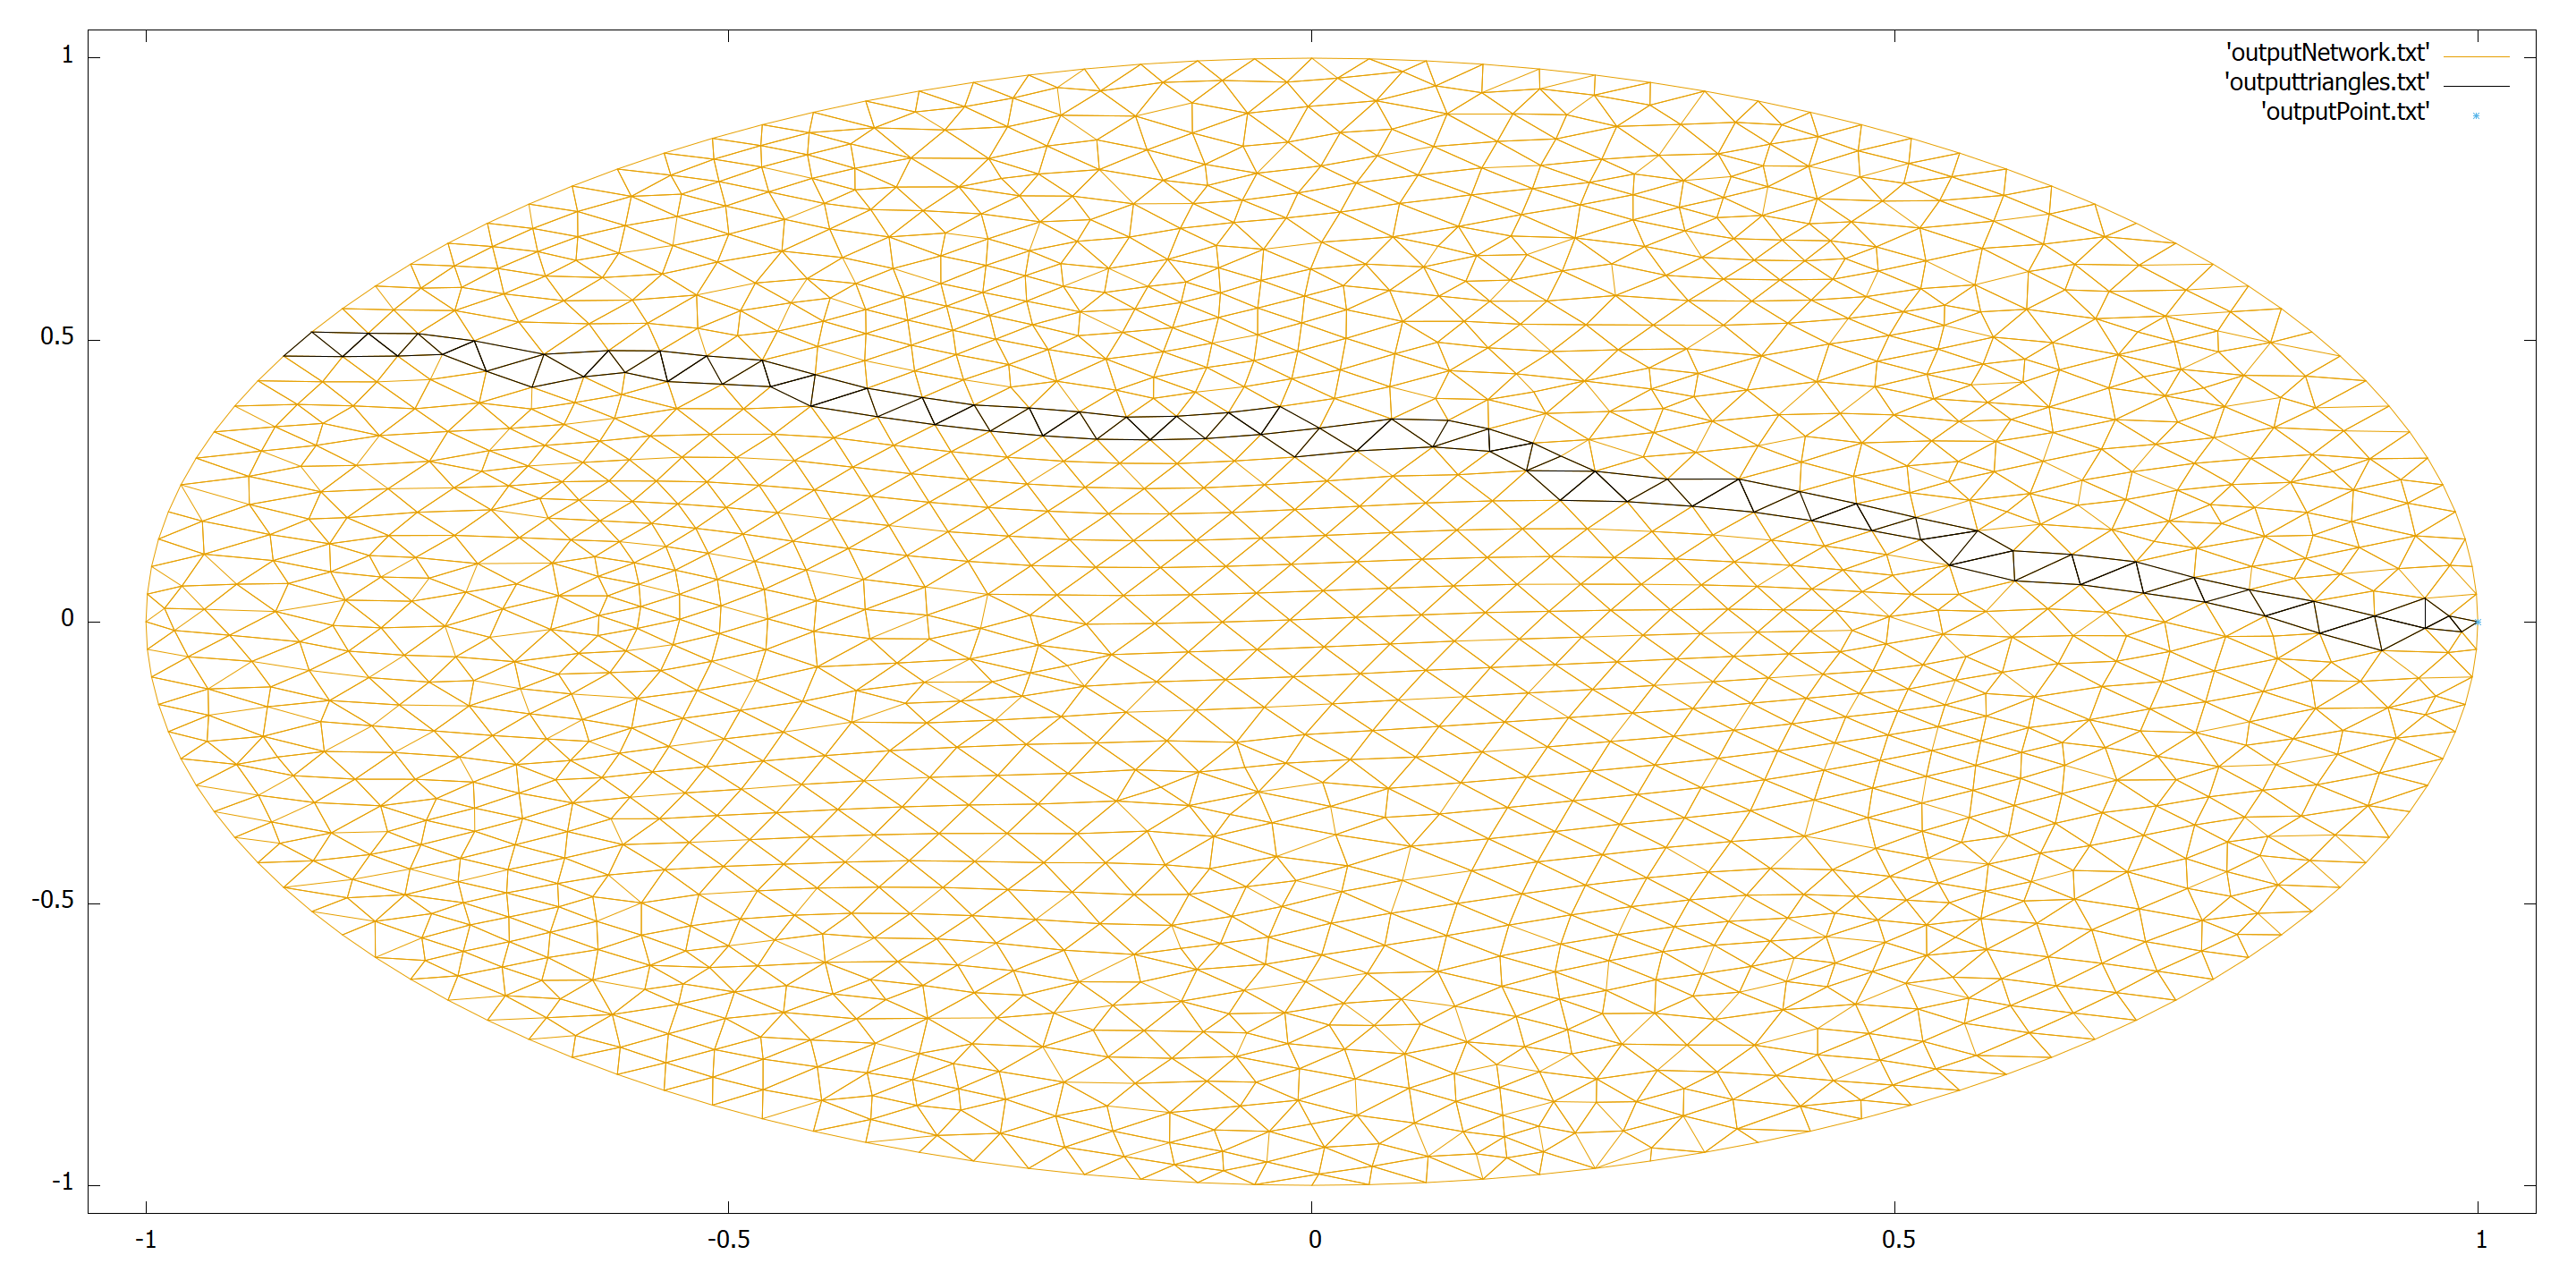
\includegraphics[width=0.55\linewidth, height=0.55\linewidth]{../Figures/StartTri600_p(1,0)_min_neg}}
%	\caption{}
	\subfigure{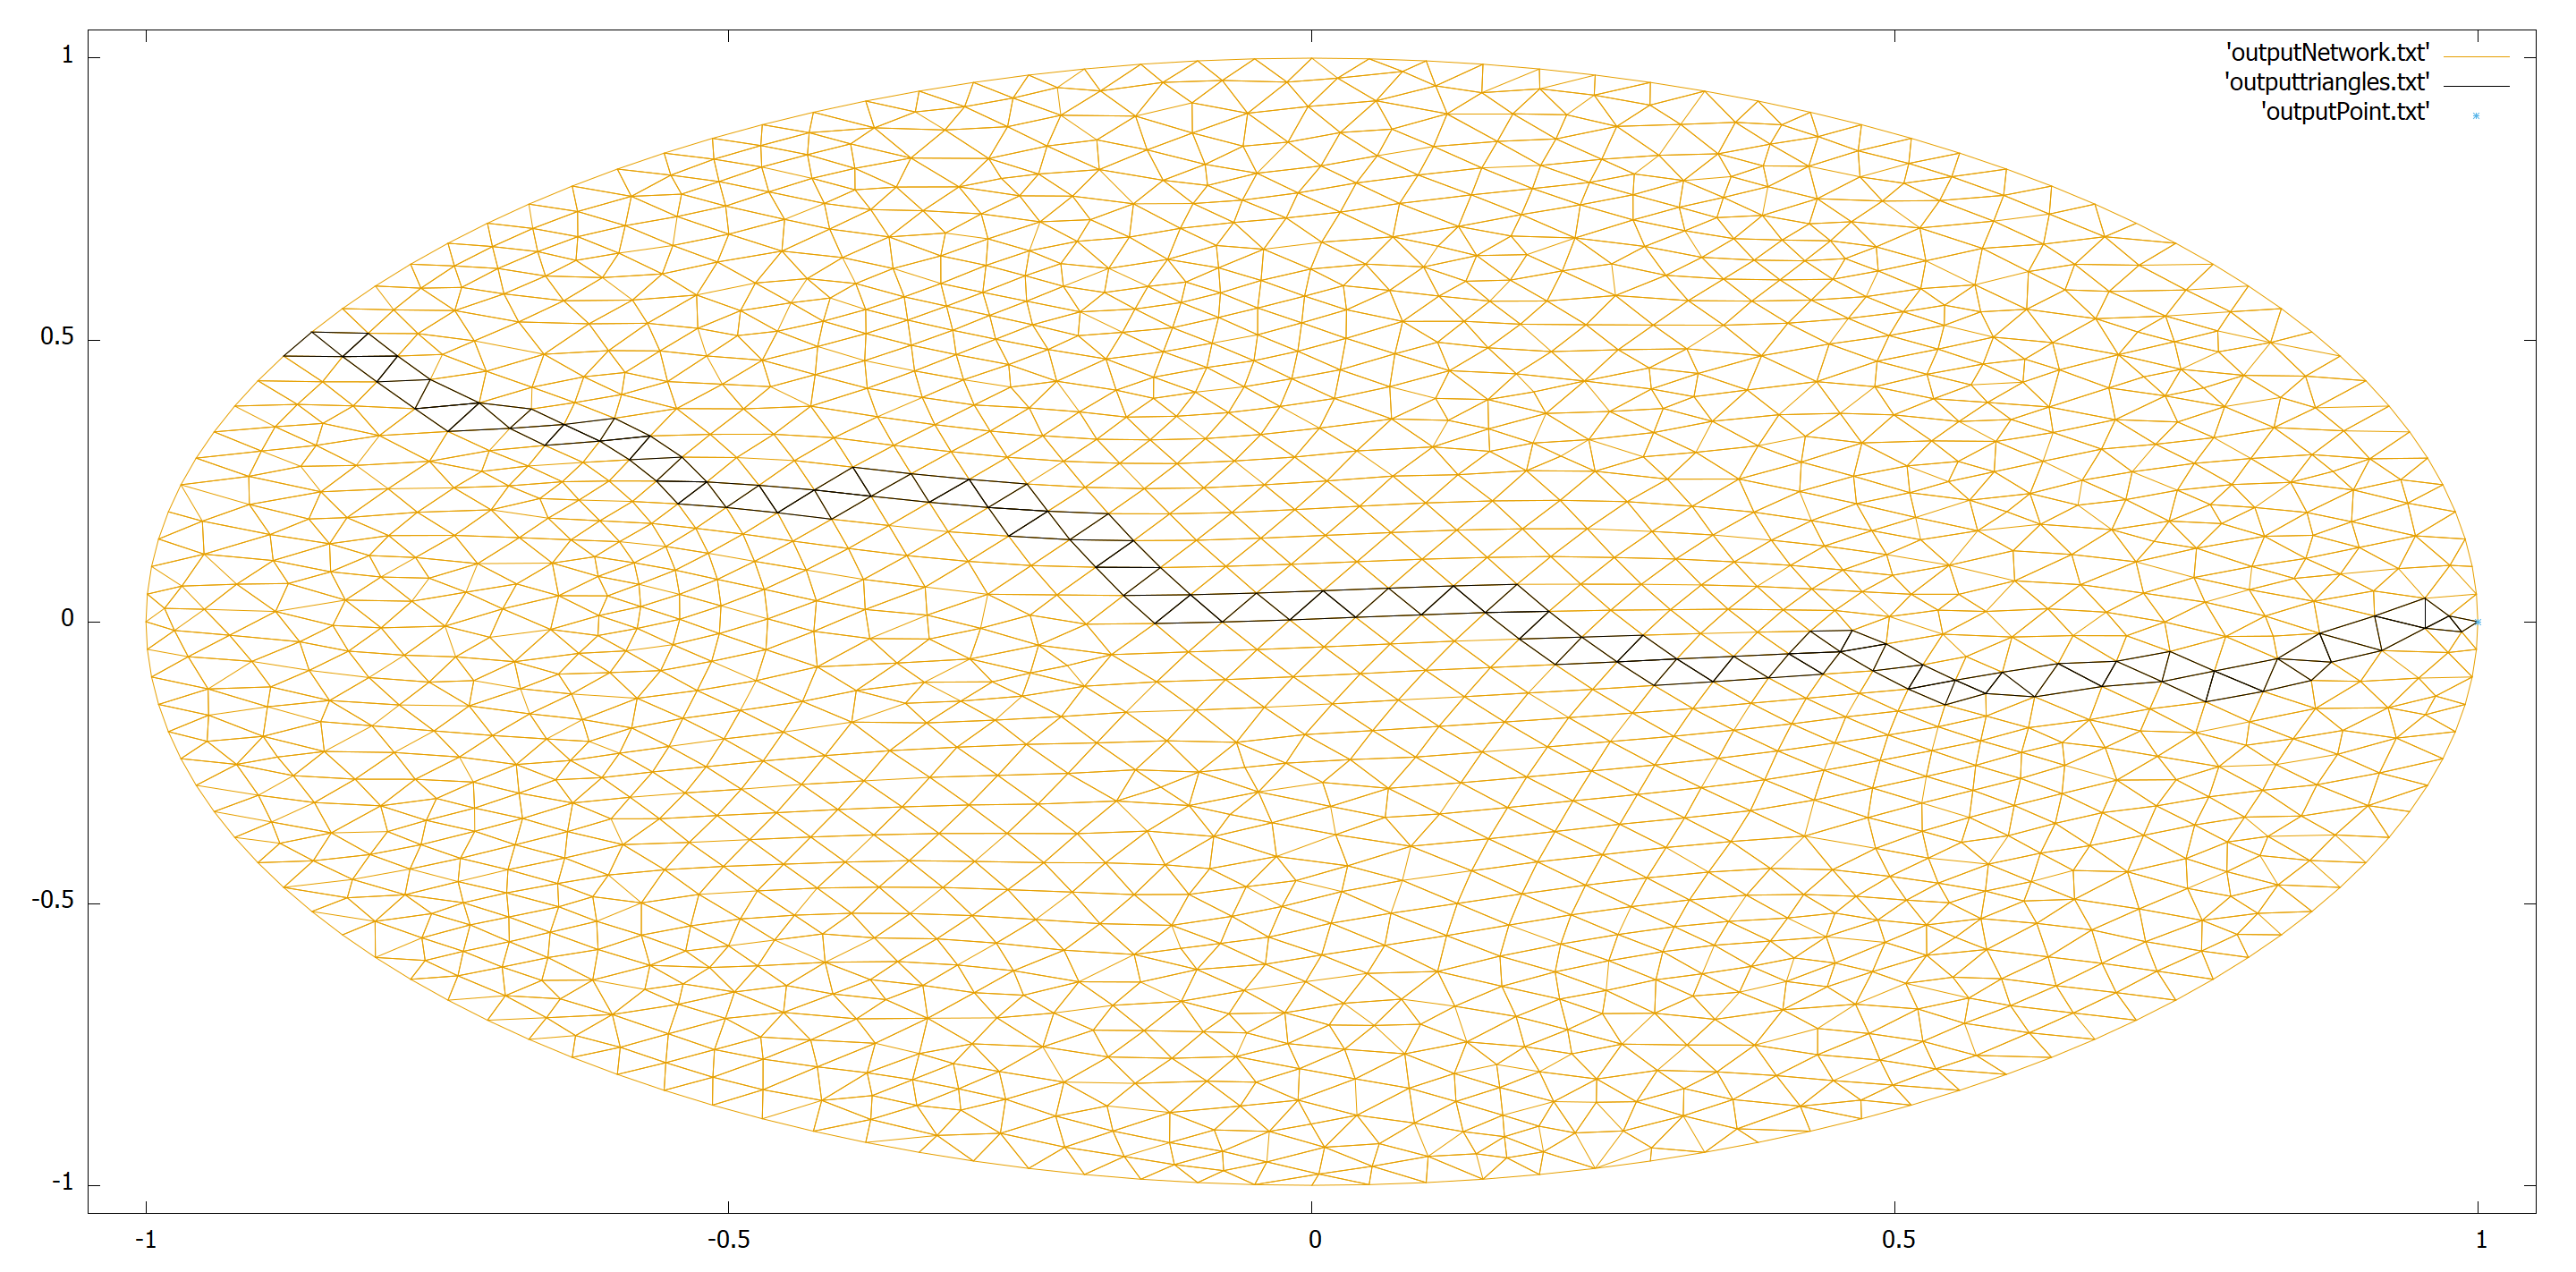
\includegraphics[width=0.55\linewidth,height=0.55\linewidth]{../Figures/StartTri600_p(1,0)_random_neg1}}
\end{figure}

\begin{figure}[h]
	\subfigure{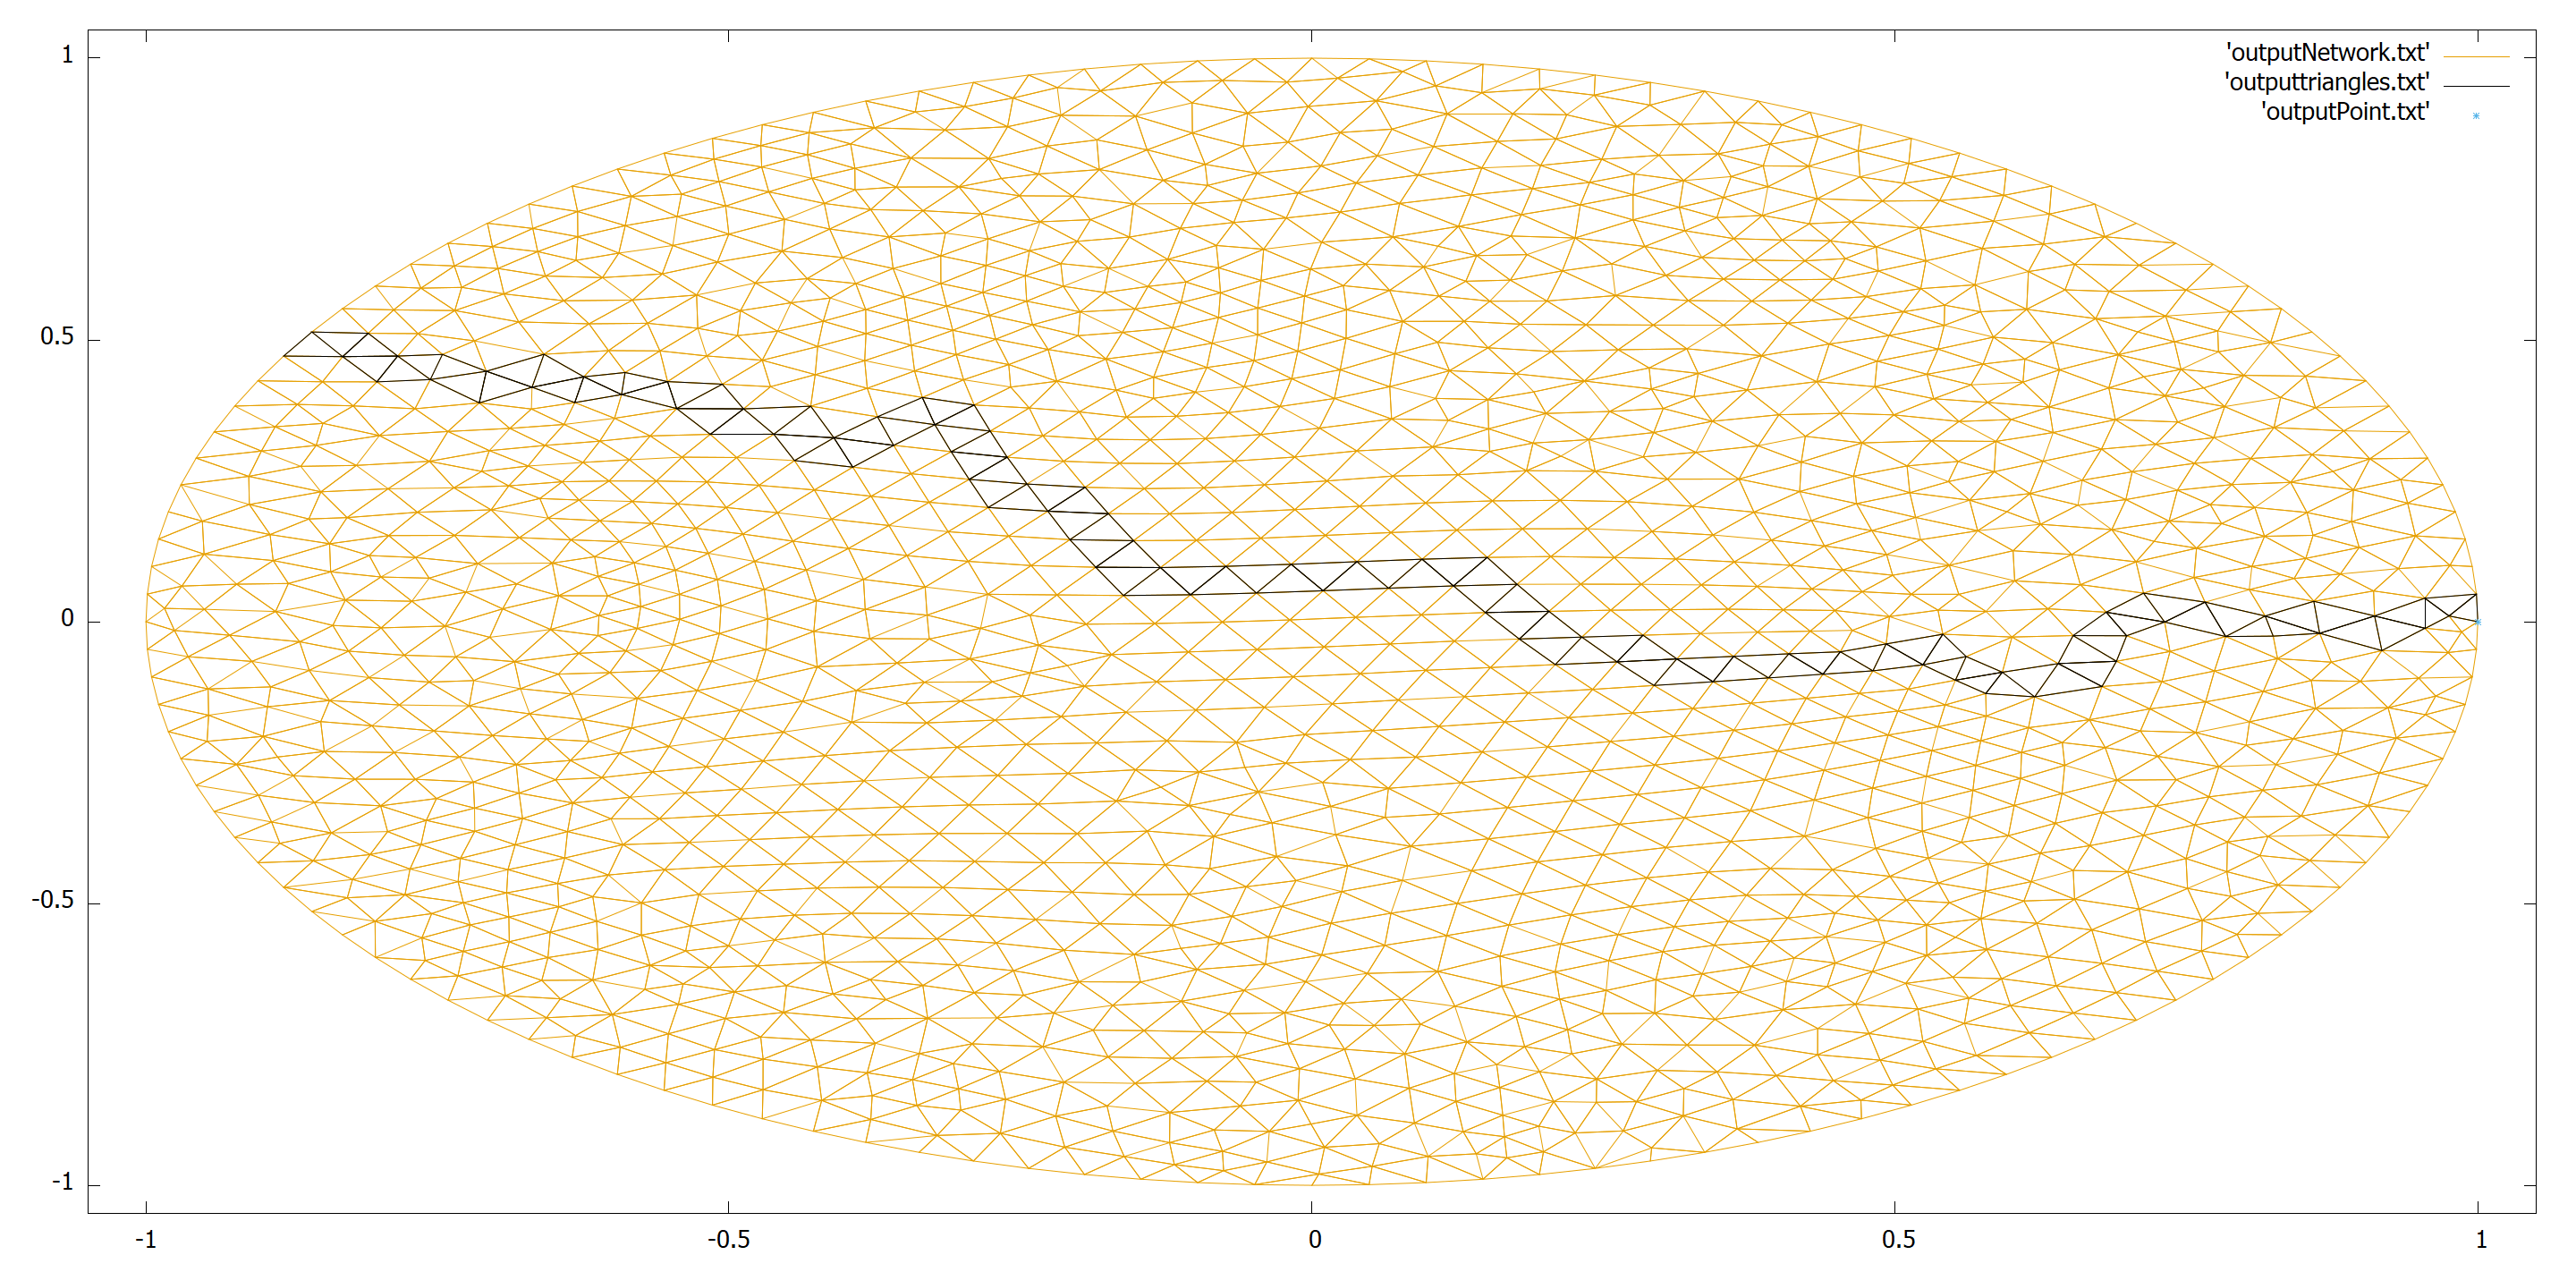
\includegraphics[width=0.55\linewidth,height=0.55\linewidth]{../Figures/StartTri600_p(1,0)_random_neg2}}
	\subfigure{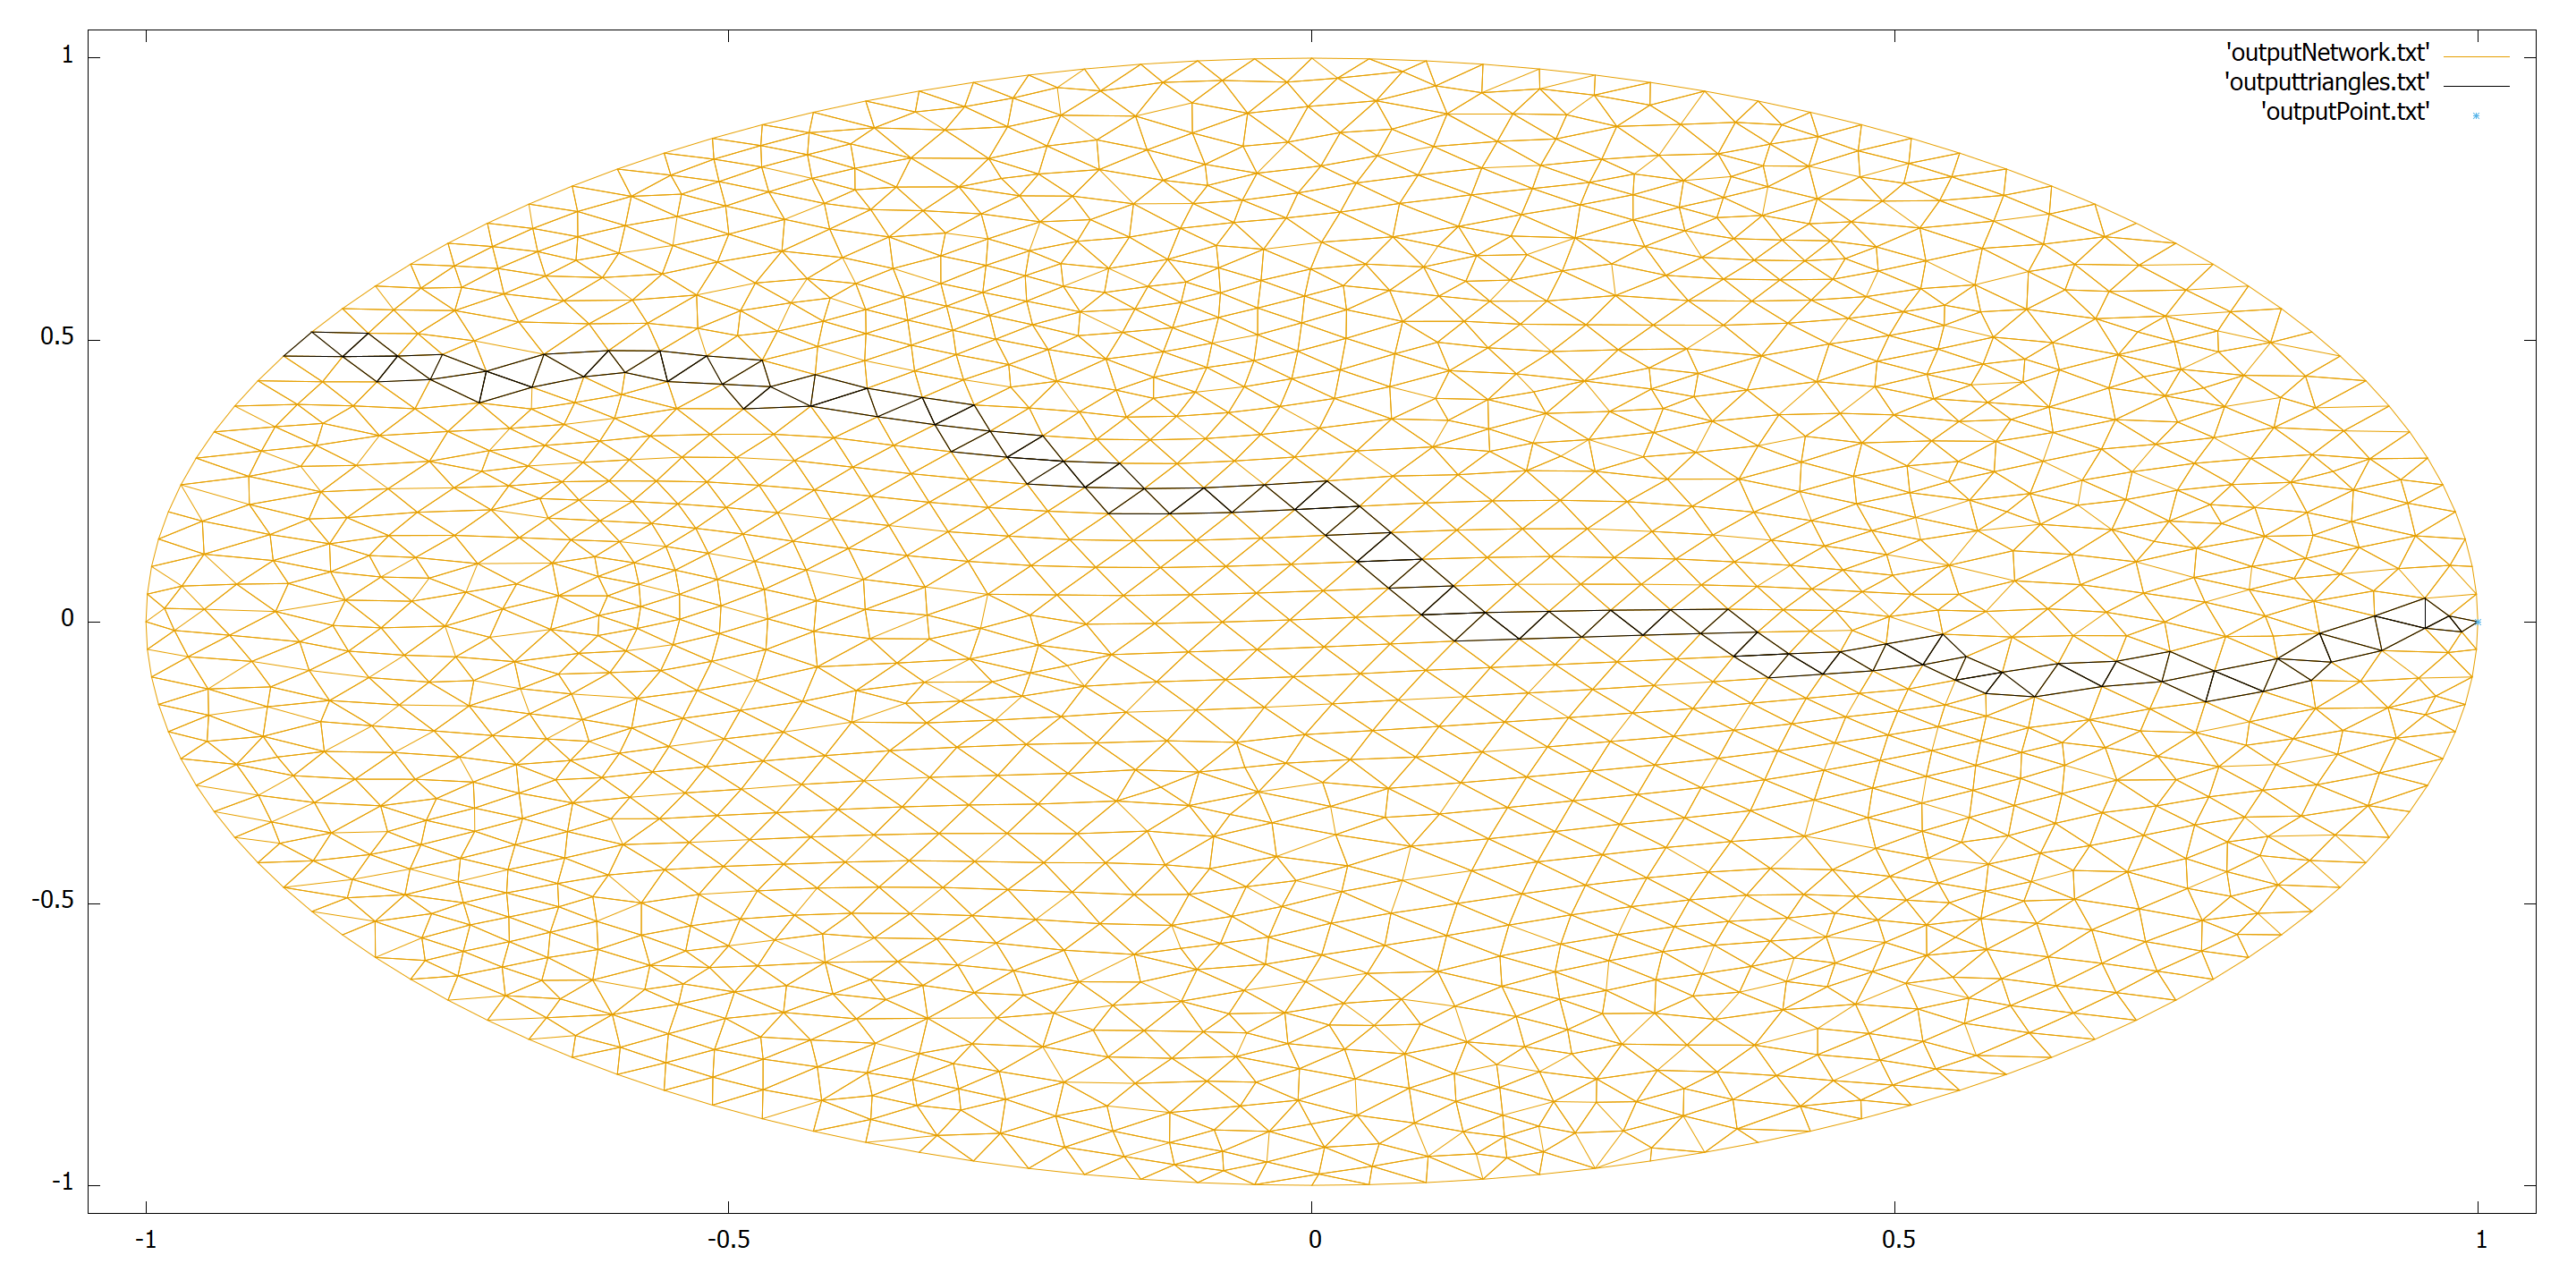
\includegraphics[width=0.55\linewidth,height=0.55\linewidth]{../Figures/StartTri600_p(1,0)_random_neg3}}
\end{figure}

\subsubsection{Can an arbitrary choice of the consecutive triangle be a better choice?}\label{Question}
	This example shows that a random choice of the consecutive triangle can be better. 
	\begin{figure}[h]\label{Example}
			\begin{minipage}{0.3\textwidth}
				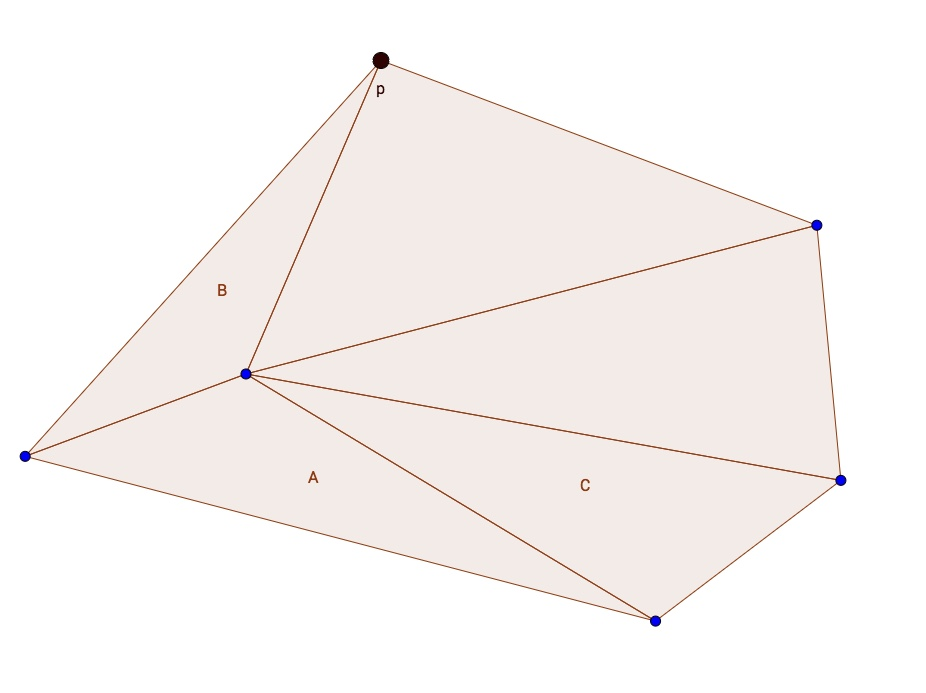
\includegraphics[scale=0.2]{../Figures/Example.jpg}
			\end{minipage}
			\hfill
			\begin{minipage}{0.4\textwidth}
				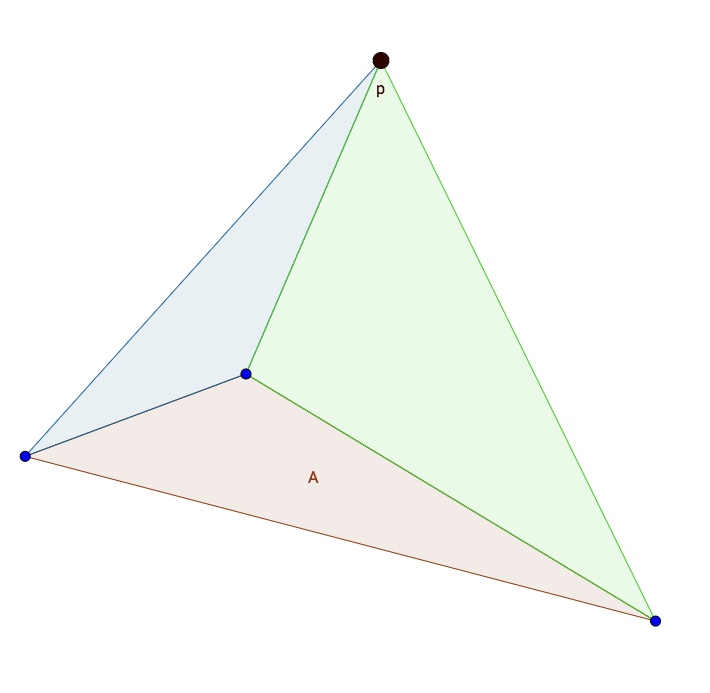
\includegraphics[scale=0.2]{../Figures/Calculation.jpg}
			\end{minipage}
		\caption{The illustration of \ref{Question}.}
			
			
	\end{figure}
	Assume that the algorithm {\ttfamily promenade} currently considers  the triangle $ A $ of Figure \ref{Example} and searches for a covering triangle of the point $ p $.
	Hence, the algorithm will proceed with triangle $ B $ or $ C $. \\
	 If we use the size of the oriented volume (the oriented volume of the convex hull of $ p $ and the lower right edge of $ A $, respectively the upper right edge of $ A $) we will clearly choose $ C $, as illustrated in the second figure (the green area is clearly bigger than the blue one). This is obviously the worse choice since $ B $ is a covering triangle of the point $ p $.  \\
	 An important observation is that the regularity of the triangles plays an important role. In this case, regularity means that all triangles of the mesh have a 'similar' area, 'similar' angles and its vertices are adjacent to a 'similar' number of triangles.
	 
	 XXX bsp erklären

\subsubsection{Empirical demonstration that the deterministic choice of the consecutive triangle is better in regular meshs}
If we take a look at the figures \ref{30} and \ref{2000} SELBE NUMMER IN PDF, it becomes empirically clear that the minimum choice of the consecutive triangle speeds up the algorithm. Figure \ref{30} even states that the path created by the minimum choice is always shorter or as long as the path created by the random choice. Looking at the runtime in \ref{2000}, we see that the runtime is about as twice as high for the random choice when the starting triangle and the given point are remote. 
 \\
Nevertheless, it has to be kept in mind that the underlying mesh plays an important role.
In this case, the mesh 'maillage5.msh', USED FOR THE CREATION OF FIGURE X, is regular in the sense explained in the previous section (see \ref{Question}).  

\begin{figure}[h] 
	\label{30}
	\subfigure{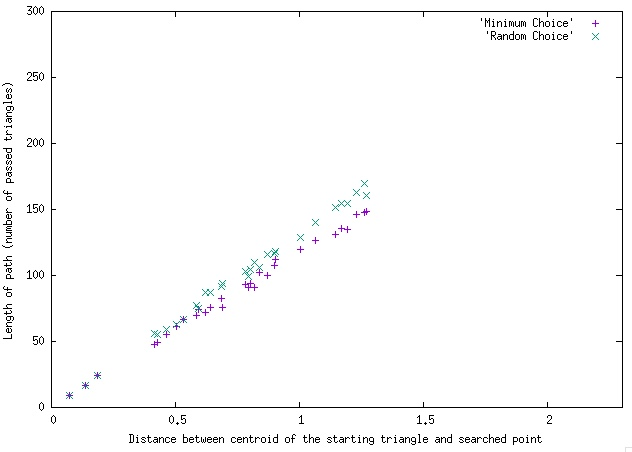
\includegraphics[width=0.8\linewidth, height=0.5\linewidth]{../Figures/Pathlength30.jpg}}
	\subfigure{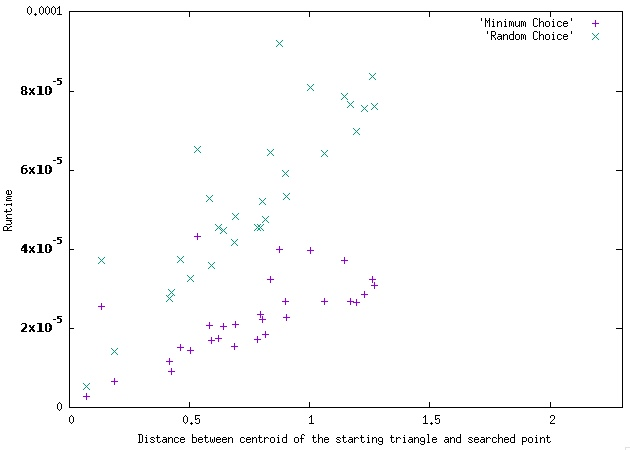
\includegraphics[width=0.8\linewidth,height=0.5\linewidth]{../Figures/Runtime30.jpg}}
	\caption{The pathlength and the runtime compared using $ min_neg $ and $ random_neg $. In this example, $ 30 $ data points were randomly created in the file 'TimeMeasurements.cpp'.  The underlying mesh is 'maillage5.msh'.}
\end{figure}

\begin{figure}[h] 
	\label{2000}
	\subfigure{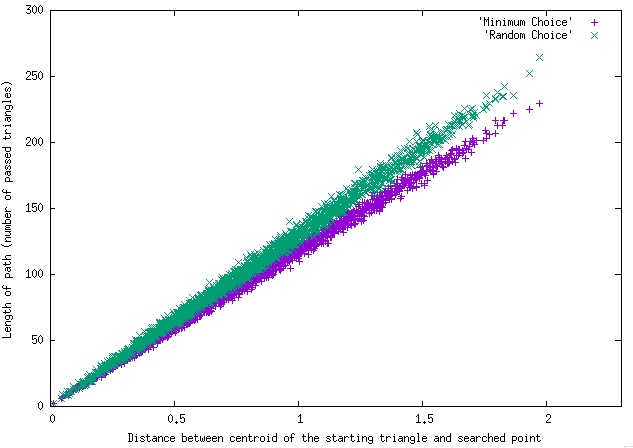
\includegraphics[width=0.8\linewidth, height=0.5\linewidth]{../Figures/Pathlength2000.jpg}}
	\subfigure{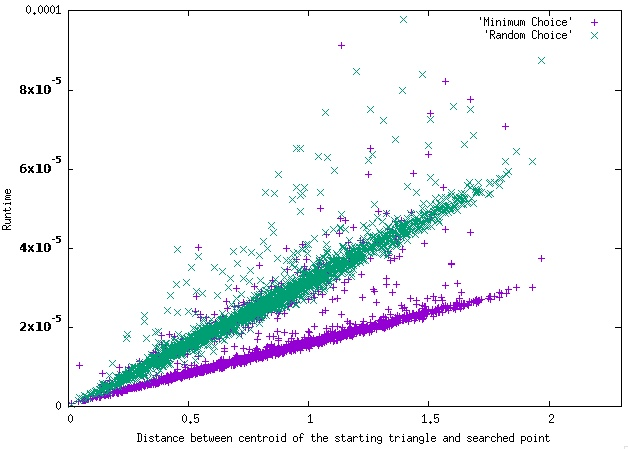
\includegraphics[width=0.8\linewidth,height=0.5\linewidth]{../Figures/Runtime2000.jpg}}
	\caption{Here, $ 2000 $ data points were randomly created.}
\end{figure}
		
		
		


\subsection{The visualization via gnuplot} \label{visualization}
	The visualization is done by the function {\ttfamily Mesh::exportGnuplot} which is able to visualize two different inputs: 
	\begin{enumerate}
		\item 
		The result of the algorithm Promenade, that is a sequence of adjacent triangles from a starting triangle to a triangle covering the searched point. 
		In this case, the input variable {\ttfamily vector<triangle> triangles\_path} contains the sequence of triangles and the input variable {\ttfamily const T3<double>* points} contains just one point, hence, the input {\ttfamily int numbpoint}, denoting the size of the array {\ttfamily points}, is $ 1 $. 
		\item 
		Given a mesh and the vertices of another mesh, it can visualize the set of the covering triangles (a subset of triangles of the first mesh) of the points of the second mesh. 
		In this case, the input variable {\ttfamily vector<triangle> triangles\_path} contains the covering triangles and {\ttfamily points} stores the vertices of the second mesh. 
	\end{enumerate}
The function writes four text files, one for all triangles of the mesh, one for the triangles in {\ttfamily triangles\_path}, one for the points in {\ttfamily points} and one for the commands which shall be executed by gnuplot. This is all realized by a simple {\ttfamily std::ofstream} variable, allowing to create and manipulate a text file. \\
The script for gnuplot contains a line which keeps the plot open until some key is hit in the terminal. 
The actual execution in the terminal is achieved by the command {\ttfamily system} which executes its input string in the terminal. XXXX The actual execution is achieved by typing the command {\ttfamily system} in the terminal. ???

\section{Cover vertices of a mesh by another mesh}

The aim of this section is to find the covering triangle for every vertex of another mesh in the same domain. This can be useful when a mesh is refined or coarsened. For this purpose, the Promenade algorithm is executed many times, once for every vertex. In order nevertheless to obtain a good running time, the starting triangle for {\ttfamily Promenade} should be chosen in an efficient way. The idea is to use starting triangles for which we already know that they are located close to the vertex to cover.

The function {\ttfamily findVertices} is given two meshes, {\ttfamily Mesh m} and {\ttfamily Mesh M}, and a reference of a vector of triangles {\ttfamily coveringTriangles} and returns {\ttfamily coveringTriangle} after modification. The function's goal is to search for covering triangles in {\ttfamily M} for the vertices of {\ttfamily  m}. At the position $i$ of {\ttfamily coveringTriangles} the triangle in {\ttfamily M} covering the $i$-th vertex of the mesh {\ttfamily m} is stored. All covering triangles are initialized by 0. Note that the indexing of the vertices in the mesh files starts at 1.

First, two random triangles, one in {\ttfamily m} and one in {\ttfamily M}, are chosen. In {\ttfamily findVertices} covering triangles for the vertices of the randomly chosen triangle {\ttfamily firstTriangle\_m = (firstVertex, secondVertex, thirdVertex)} in {\ttfamily m} are computed. In order to find a covering triangle for {\ttfamily firstVertex}, {\ttfamily Promenade} is executed given the random triangle {\ttfamily firstStartTri} chosen in the {\ttfamily M}. After calculation of the covering triangle for {\ttfamily firstVertex} indexed by {\ttfamily firstTriangle\_M}, we can use that triangle as starting triangle for the search of a covering triangle for {\ttfamily secondVertex}. As {\ttfamily firstVertex} and {\ttfamily secondVertex} belong to one edge in {\ttfamily m}, we expect the covering triangles of those vertices to be close in {\ttfamily M}. In the same manner, we use the covering triangle of {\ttfamily secondVertex} as starting triangle for covering {\ttfamily thirdVertex}. Hereby, the version of {\ttfamily Promenade} not storing the taken path is executed.\\

why start with random triangle of mesh m (JUST START WITH FIRST TRI?)\\

Now, we computed covering triangles for all the vertices of {\ttfamily firstTriangle\_m}. Originating from this triangle, we start a recurrence to find the remaining covering triangles. Neighboring triangles, neighbors of the neighboring triangles and so on will be considered.

In {\ttfamily findVertices} the function {\ttfamily Triangle\_Recurrence} is called. The two meshes, the vector {\ttfamily coveringTriangles} and the already covered triangle {\ttfamily firstTriangle\_m} are passed. {\ttfamily Triangle\_Recurrence} modifies the vector {\ttfamily coveringTriangles} and, thereafter, {\ttfamily findVertices} returns the completed vector.

{\ttfamily Triangle\_Recurrence} searches for covering triangles for the vertices of neighboring triangles of the already covered triangle. Again, 'close' covering triangle that are already found are used to accelerate the termination of the algorithm {\ttfamily Promenade}.

We start with the member {\ttfamily neighbor1} of {\ttfamily firstTriangle\_m}. If this neighbor triangle exists and its vertices are not yet covered, we do so using the same procedure as in {\ttfamily findVertices}. After the triangle is covered, we consider its member {\ttfamily neighbor1}. At the moment when either a neighbor does not exist or is already covered, we go on to the member {\ttfamily neighbor2} and afterwards to the member {\ttfamily neighbor3}. If all members are covered, we return to the calling triangle and considered its next neighbor. This terminates when a cover triangle for all vertices of the mesh {\ttfamily m} is found and the vector {\ttfamily coveringTriangles} is completed. WHY? XXXX Observe that this searching structure is similar to the approach of depth-first search. 

$selectAdjacentPoint$ to select Triangle to start {\ttfamily Promenade} (if the vertex is not already covered), then cover neighbors of this triangle


\section{Test environment- the main function}
	The cpp file main offers the possibility to test the properties of the program:
	\begin{enumerate}
		\item 
		Find the neighbors of a triangle.
		If a valid triangle index is chosen, the triangles and its neighbors are marked in the chosen mesh. This case offers the extra option to choose if the adjacency should be set via list or multimap. Essentially, the functions 
		{\ttfamily setAdjacencyViaList } or {\ttfamily setAdjacencyViaMultimap} and {\ttfamily exportGnuplot} are called. 
		\item 
		Find the covering triangle for a selectable point. 
		As a result, the path to the covering triangle of the point is displayed. 
		If the point lies outside of the mesh, the path to the nearest triangle is marked in the mesh. 
		In this case, the functions {\ttfamily Promenade} and {\ttfamily exportGnuplot} are called. 
		\item 
		Find the covering triangles for the vertices of another mesh. These option offers to display all covering triangles of a the vertices of a second mesh. Note that the mesh whose vertices is supposed to be broader (a finer mesh can be embedded in a broader mesh as well but then each triangle serves as a covering triangle). XXX DOMAIN
	\end{enumerate}
	All three options allow to choose the mesh where the mesh becomes increasingly finer from maillage1.msh to maillage5.msh. 
	Of course, it is also possible to add own meshes. In this case yet, it has to be respected that the vertex indices within a triangle must be sorted in ascending order, as mentioned in the sections before. 
	Moreover, the mesh's interval should be at maximum $ [1.5,1.5] $ for a convenient display since the axis of the plot for gnuplot are predefined as the interval $ [2,2] $.  \\
	XXXX
	The test environment is not robust face to wrong inputs. That means that, for example, if an integer is demanded but a letter is typed, the program has to be started again. The same happens if an index is demanded but a the typed input lies outside of the range (an assert exception is thrown then).  
	XXXX
	 
	special structure of mesh files is needed
	
	prepareMaillageFiles.cpp: mesh with Gmsh -> generate mesh file in required format
	
	TimeMeasurements.cpp: Figure4,5
	
	runtime of promenade ?
	
\end{document}





